\section{Backend}
\label{sec:backend}

Kod prevođenja jezika Core u neki imperativni međujezik kao što je C-\,- postoji više etapa.
Prvo se \textit{CoreSyn (GHC’s intermediate language)} prevodi u \textit{StgSyn (GHC’s intermediate language)}, i to u dve faze:
\begin{enumerate}
	\item \textbf{CoreToStg} - Core-to-Core proces konvertuje program u ANF (eng. \emph{A-normal form}). A-normalnu formu su osmislili Sabry i Fellisen 1992. god.  U ANF formi svi argumenti moraju biti trivijalni, odnosno vrednost svih argumenata se mora izračunati odmah. ANF se bavi osnovnim definicijama zasnovanim na $\lambda$ računu sa slabom redukcijom i let izrazima uz ograničenja:
	- dozvoljene su samo konstante, $\lambda$ termovi i promenljive kao argumenti funkcije
	- zahtev da rezultat netrivijalnih izraza pripada let-povezanoj promenljivoj ili vraćen iz funkcije. \\ \\
	Primer ANF: \\ f(g(x),h(y))\\
	
	\begin{tabbing}
		let v0 \= g(x) in \\
		\>let v1 \= h1(y) in \\
		\> \> f(v0, v1)
	\end{tabbing}
	
	\item \textbf{CoreToStr} - Rezultat prve faze u velikoj meri odgovara krajnjem StgSyn, zato u ovoj fazi nema preterano mnogo posla. Ova faza dekoriše StgSyn sa mnogo pomoćnih  promenljivih, let-no-escape indikatora.
	
	STG program se pomoću generatora k\^{o}da (eng. \emph{code generator}) pretvara u neki niži jezik kao što je C-\,- \cite{C--05}.
	
\end{enumerate}

\subsection{GHC k\^{o}d generator}
\label{sec:podnaslovGHCGenerator}

Glazgov Haskel Kompajler je u početku prevodio k\^{o}d za STG-mašine (eng. \emph{Spineless Tagless G-machine}) na C jezik. Ideja je bila da se iskoriste C kompajleri koji su portabilni i imaju određene dobre optimizacije. Međutim, pokazalo se da C ima mnogo mana u kontekstu jezika srednjeg nivoa (eng. \emph {intermediate language}), posebno za kompilatore lenjih funkcionalnih jezika sa nestandardnom kontrolom toka. Takođe, C ne podržava repnu rekurziju, pristup steku radi čišćenja memorije (eng. \emph{garbage collection}) i još mnogo drugih stvari. To nije iznenađujuće, jer C nije dizajniran za to. Pisci kompilatora višeg nivoa kao što je GHC su odlučili da ublaže prethodno navedene nedostatke.

Problem je trebalo da reše razne ekstenzije GNU C-a. Međutim, i ovo rešenje ima svoje mane kao što je velika zavisnost od GNU C verzije kompilatora. Optimizacija za C često nema efekta na te jezike višeg nivoa - mnogo statičkih informacija bi moglo biti izgubljeno. 

Kao odgovor na to, GHC je ubacio podršku za k\^{o}d generatore niskog nivoa (eng. \emph{native code generators}), koji direktno prevode u mašinski k\^{o}d, ali samo za određene sisteme, konkretno x86, SPARC, PowerPC.

Želja da se zadrže dobre osobine svođenja i kompajliranja na C, a da se opet prevaziđu problemi, inspirisala je razvoj jezika srednje-niskog nivoa (eng. \emph{low-level intermediate languages}). Od interesa je jezik C-\,-, jer je dizajniran pod uticajem GHC-a. Iako je upotreba jezika C-\,- kao srednjeg jezika tehnički veoma perspektivan pristup, dolazi sa velikim praktičnim problemima: razvoj portabilnog kompilatorskog bekenda je isplativ, ako ga koristi više kompilatora, a pisci kompilatora ne žele da rade na razvoju nečega što neće biti u širokoj upotrebi. Kao posledica toga, neka varijanta C-\,- jezika se koristi kao srednje-niski jezik u GHC-u, ali generalno nema razvijenog bekenda u jeziku C-\,- koja bi mogla biti podržana od strane većeg broja kompilatora kao što je GHC \cite{SPJ92}.

Navodimo tri najznačajnija programa za generisanje izvršnog k\^{o}da:
\begin{enumerate}
	\item  NGC (eng. \emph{Native Generated Code}): kao prvo rešenje odgovara generisanju asemblerskog k\^{o}da. To se pokazalo kao brzo i efikasno rešenje, ali je imalo i veliki nedostatak, jer se za svaku platformu računara (x86, SPARC, PowerPC, ...) morao održavati pripadni asemblerski k\^{o}d.
	NCG sadrži 20,570 linija k\^{o}da, što je približno 4 puta više od veličine k\^{o}da C-kompajlera. Pritom je kompilacija bila dvostruko brža. Jedna od prednosti NCG u odnosu na C je jednostavnost; iako je NCG k\^{o}d mnogo veći, sigurno je i mnogo jednostavniji.
	\item  C-\,- : drugo rešenje se našlo u programskom jeziku C-\,-, podskupu jezika C, specijalno prilagođenom zadacima kompilacije. Jedna od apstrakcija koju C-\,- nudi su virtualni registri. Oni omogućavaju mapiranje mašinskih registara na optimalan način. Delimično u tome učestvuje i run-time verzija GHC-a. C-\,- verzija kompajlera se znatno razlikuje od zvaničnog C-\,- standarda. Osnovna razlika je u  implementaciji sopstvenog GC-a (eng. Garbage Collector), jer Haskel zahteva GC koji je generacijski i koji može da radi po blokovima hipa odnosno steka. Generacijski GC polazi od pretpostavke da će najnoviji objekti biti najbrže skidani sa hipa odnosno steka, stoga se GC primenjuje samo na najmlađu generaciju objekata, a tek kada to ne daje zadovoljavajući rezultat, onda se analiziraju i starije generacije. Na slici \ref{fig:cmm} je prikazan k\^{o}d u C-\,- koji, očigledno, u velikoj meri liči na C k\^{o}d. 
	\item LLVM : trenutno je najperspektivniji bekend frejmvork-okvir (eng. \emph{framework}), koji dolazi sa just-in-time kompilacijom (kojom se kompajliraju samo delovi k\^{o}da koji su ispravljani nakon poslednjeg kompajliranja) kao i life-long analizom (dubinskom analizom za dobijanje optimalnog k\^{o}da).
	
	Postoje četiri osnovna razloga za njegovu implementaciju \cite{Ter10}:
	\begin{itemize}
		\item Pravljenje kompajlera visokih performansi za generisanje k\^{o}da zahteva mnogo uloženog truda i znanja. Tako, razvoj LLVM-a je počeo pre oko 15 godina. Postojanje ovakvog sistema će zahtevati mnogo manje posla na održavanju i proširenju, nego što prethodna dva rešenja zahtevaju. Takođe, pošto je LLVM nezavisan projekat, buduća poboljšanja će biti automatski raspoloživa. 
		\item GHC proizvodi Haskel programe koji se brzo izračunavaju. Međutim, mnoge optimizacije na nižem nivou (naročito one koje podrazumevaju poznavanje specifičnosti arhitekture računara) nisu do kraja implementirane. Korišćenjem LLVM-a, koji koristi mnoge specifičnosti arhitektura računara, ćemo ih automatski dobiti.
		\item Bitna osobina LLVM-a je ta što je od početka dizajniran kao sredina za razvoj kompajlera. Tako je moguće, u kratkom vremenskom roku i sa relativno malo truda, realizovati prilagođavanje svake nove verzije LLVM-a postojećoj aplikaciji GHC-a. 
		\item LLVM je projekat koji uključuje celokupan lanac alata sa C/C++ kompajlerom, asemblerskim alatima, linkerom, debagerom i alatima za statičku analizu. Koristi se za više programskih jezika, pa mu je baza korisnika garancija da će se i u buduće kvalitetno razvijati. 
	\end{itemize}
\end{enumerate}


\begin{figure}[h!]
	\begin{center}
		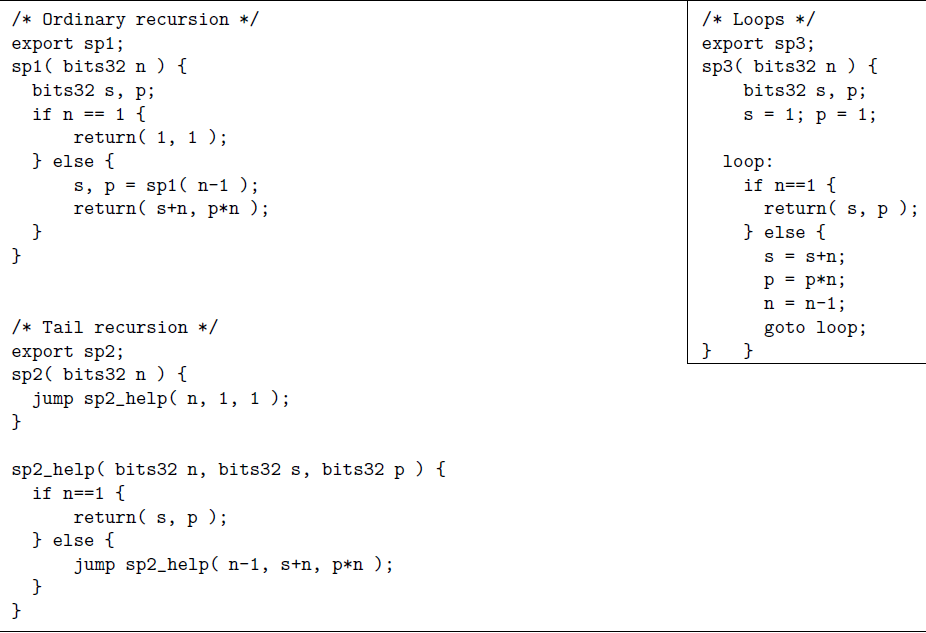
\includegraphics[scale=0.40]{resources/cmm.png}
	\end{center}
	\caption{Tri funkcije za izračunavanje sume i proizvoda prvih n brojeva u programskom jeziku C-\,-}
	\label{fig:cmm}
\end{figure}

Prikažimo rezultate korišćenja LLVM-a na jednostavnom primeru izračunavanja funkcije zadate na sledeći način:
\begin{itemize}
	\item ako je n parno, sledeći broj je n/2
	\item ako je n neparno, sledeći broj je 3*n+1
	\item ako je n jedan, stop
\end{itemize}

Cilj je da nađemo najdužu sekvencu za početne brojeve od jedan do milion. Sekvencu čini broj koraka dok ne stignemo do stopa. Kod napisan u Haskelu je:

\begin{verbatim}
import Data.Word

collatzLen :: Int -> Word32 -> Int
collatzLen c 1 = c
collatzLen c n | n `mod` 2 == 0 = collatzLen (c+1) $ n `div` 2
| otherwise      = collatzLen (c+1) $ 3*n+1

pmax x n = x `max` (collatzLen 1 n, n)

main = print . solve $ 1000000
where solve xs = foldl pmax (1,1) [2..xs-1]
\end{verbatim}

Kompilacijom ovog k\^{o}da različitim vrstama generisanja izvršnog k\^{o}da, dobijaju se vremena prikazana u tabeli \ref{tab:vremena}.

\begin{table}[h!]
	\begin{center}
		\caption{Različita vremena generisanja izvršnih k\^{o}dova}
		\begin{tabular}{||c|c|c|c||} \hline
			GHC-6.13 (NCG) & GHC-6.13 (C) & GHC-6.13 (LLVM) & GCC-4.4.3 \\ \hline
			2.876s & 0.576s & 0.516s & 0.335s \\ \hline
		\end{tabular}
		\label{tab:vremena}
	\end{center}
\end{table}


Iako se očekuje da NCG  ima najkraće vreme izvršavanja, jer se direktno prevodi na mašinski k\^{o}d, vidimo da u ovom jednostavnom primeru to nije slučaj.

Prethodni primer se može jednostavno paralelizovati. Odgovarajući Haskel k\^{o}d je:

\begin{verbatim}
import Control.Parallel
import Data.Word

collatzLen :: Int -> Word32 -> Int
collatzLen c 1 = c
collatzLen c n | n `mod` 2 == 0 = collatzLen (c+1) $ n `div` 2
| otherwise      = collatzLen (c+1) $ 3*n+1

pmax x n = x `max` (collatzLen 1 n, n)
main = print soln
where
solve xs = foldl pmax (1,1) xs
s1 = solve [2..500000]
s2 = solve [500001..999999]
soln = s2 `par` (s1 `pseq` max s1 s2)
\end{verbatim}

U programu je jednostavno ostvarena podela na dva dela i kombinovanje korišćenjem Haskelovih 'par' i 'pseq' funkcija, koje ukazuju kompajleru da paralelno realizuje dva dela s1 i s2. U ovom slučaju, vreme izvršavanja pomoću LLVM-a je:

GHC-6.13 (Parallel, LLVM): 0.312

%STG-mašina se koristi za mapiranje ne-striktnih funkcionalnih jezika u hardver računara. Razvijena je za potrebe GHC kompajlera, u kom se intenzivno koristi. Realizovana je kao interpreter, sa ciljem da bude jednostavna za analizu i korišćenje (eng. user-friendly). Neki autori smatraju STG-mašinu kao deo međujezika zajedno sa Core-om.
%Pun naziv STG-mašine (eng. Spineless Tagless Graph Reducing Machine) je nastao od pojmova G-mašina koja ima apstraktnu arhitekturu za obradu programa na funkcionalnom jeziku i pojmova: 
%spineless ukazuje da graf nije prikazan kao jedinstvena struktura podataka u memoriji, već kao skup manjih pojedinačnih delova grafa koji se međusobno referišu. Značajan deo mehanizma evaluacije čini deo koji se odnosi na referisanje tih delova.
%tagless ukazuje da su sve vrednosti na hipu (neizračunati izrazi, funkcije, već izračunati izrazi) prikazane na sličan način kroz zatvorenja (eng. closure). Ovo je obrnuto od tagfull, gde su zatvorenja anotirana podacima o tipu izraza i da li je izraz već izračunat.
%graph reducing ukazuje da izrazi na hipu mogu biti prepisani jednostavnijim vrednostima koje mašina smatra ekvivalentim početnom izrazu. Na primer, izračunavanje izraza 1+1 na hipu, može biti zamenjeno konstantom 2, pritom taj rezultat (2) je eventualno ostvaren na nekom drugom mestu.
%Ideja ove mašine je da predstavi program u formi apstraktnog sintaksnog drveta. Međutim, zbog referisanja delova sintaksnog drveta, program je u obliku grafa, a ne drveta. Evaluacijom tog grafa, korišćenjem malog broja instrukcija, sistematski ga redukujemo do krajnjeg oblika, što će biti rezultat izvršavanja programa.

%
%\begin{primer} Ovako se ubacuje slika. Obratiti pažnju da je dodato i 
%	\begin{verbatim}
%	\usepackage{graphicx}
%	\end{verbatim}
%	
%	\begin{figure}[h!]
%		\begin{center}
%			%\includegraphics[scale=0.75]{panda.jpg}
%		\end{center}
%		\caption{Pande}
%		\label{fig:pande}
%	\end{figure}
%	
%	Na svaku sliku neophodno je referisati se negde u tekstu. Na primer, na %slici \ref{fig:pande} prikazane su pande. 
%\end{primer}
%
%\begin{primer} I tabele treba da budu u svom okruženju, i na njih je neophodno referisati se u tekstu. Na primer, u tabeli% \ref{tab:tabela1} su prikazana različita poravnanja u tabelama.
%	
%	\begin{table}[h!]
%		\begin{center}
%			\caption{Razlčita poravnanja u okviru iste tabele ne treba koristiti jer su nepregledna.}
%			\begin{tabular}{|c|l|r|} \hline
%				centralno poravnanje& levo poravnanje& desno poravnanje\\ \hline
%				a &b&c\\ \hline
%				d &e&f\\ \hline
%			\end{tabular}
%			\label{tab:tabela1}
%		\end{center}
%	\end{table}
%	
%\end{primer}